\documentclass{vldb}

\usepackage{latexsym}
\usepackage{amsmath}
\usepackage{algorithmic}
\usepackage{algorithm}
\usepackage{clrscode}
\usepackage{graphics}
%\usepackage{epsfig}
%\usepackage{epic}
%\usepackage{eepic}
%\usepackage{xspace}
\usepackage{pst-tree}

%\addtolength{\textwidth}{1in}
%\addtolength{\oddsidemargin}{-0.5in}
%\addtolength{\evensidemargin}{-0.5in}
%\addtolength{\textheight}{0.8in}
%\addtolength{\topmargin}{-0.5in}
%\leftmargini 2.9ex


\def\punto{$\hspace*{\fill}\Box$}
\newcommand{\nop}[1]{}
\newcommand{\tuple}[1]{{\langle#1\rangle}}
\def\lBrack{\lbrack\!\lbrack}
\def\rBrack{\rbrack\!\rbrack}
\newcommand{\Bracks}[1]{\lBrack#1\rBrack}


\newtheorem{theorem}{Theorem}[section]
\newtheorem{metatheorem}{Metatheorem}[section]
\newtheorem{example}[theorem]{Example}
%\newtheorem{algorithm}[theorem]{Algorithm}
\newtheorem{definition}[theorem]{Definition}
\newtheorem{proposition}[theorem]{Proposition}
\newtheorem{property}[theorem]{Property}
\newtheorem{corollary}[theorem]{Corollary}
\newtheorem{lemma}[theorem]{Lemma}
\newtheorem{remark}[theorem]{Remark}
\newtheorem{conjecture}[theorem]{Conjecture}
\newtheorem{proviso}[theorem]{Proviso}
\newtheorem{todo}[theorem]{ToDo}

\newcommand{\comment}[1]{}
\newcommand{\compiler}{DBToaster}

\title{\compiler: A SQL Compiler for High-Performance Delta Processing in
Main-Memory Databases}
\author{Yanif Ahmad and Christoph Koch \\
Department of Computer Science \\ Cornell University, Ithaca, NY \\
\{yanif, koch\}@cs.cornell.edu}
\date{}


\begin{document}


\maketitle

\begin{abstract}
We present \compiler, a novel query compilation framework for producing high
performance compiled query executors that incrementally and continuously answer
standing aggregate queries using in-memory views. \compiler\ targets applications
that require efficient main-memory processing of standing queries
(\textit{views}) fed by high-volume data streams, \textit{recursively} compiling
view maintenance (VM) que\-ries into simple C++ functions for evaluating database
updates (\textit{deltas}).
While today's VM algorithms consider single deltas on view queries to produce
maintenance queries, we recursively consider deltas of maintenance queries and
compile to thoroughly transform queries into code. Recursive compilation
successively elides certain scans and joins, and eliminates significant query
plan interpreter overheads.
\comment{
Our compilation process models and implements group-by aggregates as
an associative map data structure, and obtains procedures to update these maps by
applying a set of map expression rewrites, which can then easily be turned into
C++ code.
}

In this demonstration, we walk through our compilation algorithm, and show the
significant performance advantages of our compiled executors over other query
processors. We are able to demonstrate orders of magnitude improvements in
processing times for a financial application and a data warehouse loading
application over PostgreSQL, HSQLDB, a commercial DBMS, System 'A', the Stanford
STREAM engine, and a commercial stream processing engine 'B'.
\end{abstract}




In recent years, algorithmic trading systems have come to account for a majority
of volume traded at the major US and European financial markets (for instance,
for 73\% of all US equity trading volume in the first quarter of 2009
\cite{Iati2009}). The success of automated trading systems depends critically on
strategy processing speeds: trading systems that react faster to market events
tend to make money at the cost of slower systems. Unsurprisingly, algorithmic
trading has become a substantial source of business for the IT industry; for
instance, it is the leading vertical among the customer bases for high-speed
switch manufacturers (e.g., Arista \cite{Becht2010}) and data stream processing.




A typical algorithmic trading system is run by mathematicians who develop
trading strategies and by programmers and systems experts who implement these
strategies to perform fast enough, using mainly low-level programming languages
such as C. Developing trading strategies requires a feedback loop of simulation,
back-testing with historical data, and strategy refinement based on the insights
gained. This loop, and the considerable amount of low-level programming that it
causes, is the root of a very costly {\em productivity bottleneck}\/: in fact,
the number of programmers often exceeds the number of strategy designers by
an order of magnitude.


Trading algorithms often perform a considerable amount of data crunching
and statistical processing that could in principle be implemented using SQL
views, coupled with some relatively straightforward control and trading logic.
%
Differently from other areas of finance such as technical analysis,
where stream processing engines
\cite{abadi-vldbj:03,motwani-cidr:03} can be applied,
data processing in trading algorithms using views cannot be performed by DBMS or
data stream processing systems today: the former are not able to (1) {\em update
their views at the required rates}\/ (for popular stocks, hundreds of orders per
second may be executed, even outside burst times) and the latter are not able to
(2) {\em maintain large enough data state}\/ and support suitable query
languages (non-windowed SQL aggregates) on this state.

%
A data management system that could handle these two requirements would yield a
very substantial productivity increase that can be directly monetized -- the
holy grail of algorithmic trading.

Trading algorithms often perform a considerable amount of data crunching that
could in principle be implemented as SQL views, but cannot be achieved by DBMS
or data stream processing systems today: DBMS are not able to (1) {\em update
their views at the required rates}\/ (for popular stocks, hundreds of orders per
second may be executed, even outside burst times) and stream engines are not
able to (2) {\em maintain large enough data state}\/ and support suitable query
languages (non-windowed SQL aggregates) on this state.
A data management system fulfilling these two requirements would yield a very
substantial productivity increase that can be directly monetized -- the holy
grail of algorithmic trading.



To understand the need to maintain and query a large data state, note that
many stock exchanges provide a detailed view of the market microstructure
through complete bid and ask {\em limit order books}. The bid order book is a
table of purchase offers with their prices and volumes, and correspondingly the
ask order book indicates investors' selling orders. Exchanges execute trades by
matching bids and asks by price and favoring earlier timestamps. Investors
continually add, modify or withdraw limit orders, thus one may view order books
as relational tables subject to high update volumes. The availability of order
book data has provided substantial opportunities for automatic algorithmic
trading.





To illustrate this, we describe the Static Order Book Imbalance (SOBI) trading
strategy. SOBI computes a volume-weighted average price (VWAP) over those orders
whose volume makes up a fixed upper $k$-fraction of the total stock volume in
both bid and ask order books. SOBI then compares the two VWAPs and, based on
this, predicts a future price drift (for example a bid VWAP larger than an ask
VWAP indicates demand exceeds supply, and prices may rise). For simplicity, we
present the VWAP for the bids only:



\begin{verbatim}
select avg(b2.price * b2.volume) as bid_vwap
from   bids b2
where  k * (select sum(volume) from bids)
         > (select sum(volume) from bids b1
            where b1.price > b2.price);
\end{verbatim}
\comment{
Focusing on the $k$-fraction of the order book closest to the current price
makes the SOBI strategy less prone to attacks known as {\em axes}\/ (large
tactical orders far from the current price that will thus not be executed but
may confuse competing algorithms).
}


Coming back to our two desiderata, for trading algorithms to be successful, (1)
views such as VWAP need to be maintained and monitored by the algorithms at or
close to the trading rate. However, (2) the views cannot be expressed through
time-, row- or punctuation-based window semantics.




\begin{figure}
\begin{center}
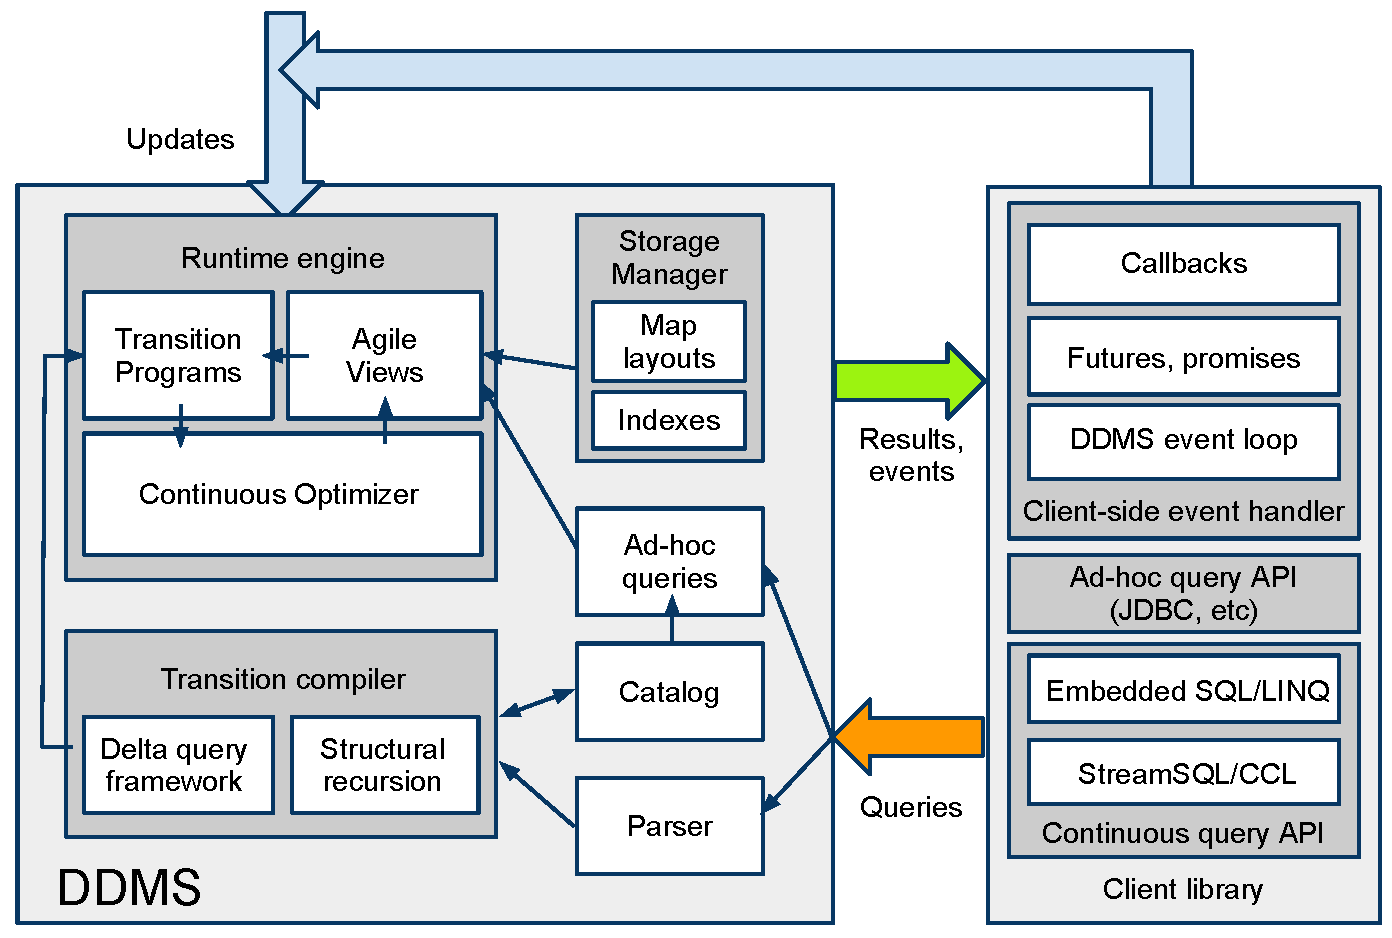
\includegraphics[width=3.3in]{graphics/CIDRarch.pdf}
\end{center}
\vspace*{-0.2in}
\caption{Dynamic Data Management System (DDMS) and Application Interface
Architecture}
\label{fig:ddmsarch}
\vspace*{-0.2in}
\end{figure}

We now examine the architecture of a DDMS, as illustrated in Figure
\ref{fig:ddmsarch}.  The core component of a DDMS is its runtime engine.  Unlike
a traditional database system where the same engine manages all database
instances, each individual DDMS execution runtime is constructed around a
specific set of queries provided by the client program (e.g., via SQL code
embedded inline in the program), each defining an \textit{agile view}.

\subsection{Application Interfaces}

The data that is processed by a DDMS arrives at the system in the form of an
update stream of tuple insertions, deletions and modifications. The stream need
not be ordered in any shape or form, and deletions are assumed to apply to
tuples that have already been seen at some arbitrary prior point on the stream.
Updates are fully processed on-the-fly, and their effects on agile views are
realised in atomic fashion, prior to working on any subsequent update. Depending
on the type of results requested by queries, any results arising from updates
will be directly forwarded to application code as agile views are maintained.

DBToaster provides a wide variety of client interfaces to issue queries and
obtain results from the DDMS, to reflect the diverse needs of applications built
on top of our tool. Today's stream processors tend to be black-box systems that
run completely decoupled from the application. Client libraries interact with
stream processors through remote procedure call abstractions, issuing queries
and new data through function calls, and either polling or being notified
whenever results appear on a queue that is associated with a TCP socket
connected to the stream processor.

In DBToaster, the set of agile views requested by clients, the \textit{visible
schema}, forms the primary read interface between client programs and the DDMS
runtime. Clients can submit queries for which the DDMS materializes an agile
view through three methods:
(1) a continuous query client API, as done with existing stream client
libraries, which sends a query string to the DDMS server for parsing,
compilation, and agile view construction. The query string may be specified in a
standard streaming language such as StreamSQL or CCL~\cite{jain-pvldb:08}. The
client may specify several ways to receive results, as seen below.
(2) an ad-hoc query client API, which issues a one-time query to the
DDMS, and returns the agile view as a datastructure to be used by the remainder
of the client program. This API may be used in both synchronous and
asynchronous modes, as indicated by the type of result requested. The query is
specified in standard SQL.
(3) an embedded language, whose syntax and data model are natural fits to the
host language in which the client application is written. Examples include
embedded SQL, and collection comprehension oriented approaches such as LINQ,
Links, and Ferry~\cite{meijer-sigmod:06,cooper-fmco:06,grust-sigmod:09}.
One interesting challenge with the embedded language approach is that of
enabling asynchronous event-driven programming. Whereas language embeddings
are natural for ad-hoc querying, we have yet to see these approaches
for stream processing.

Given these modes of issuing queries to the DDMS, our client interface supports
four methods of receiving results:
(1) callbacks, that can be specified as handlers as part of the continuous query
API. Callbacks receive a stream of query results, and are the simplest form of
result handlers that run to completion on query result events.  
(2) a DDMS event loop, which multiplexes result streams for multiple queries.
Applications may register callbacks to be executed on any result observed on the
event loop, allowing complex application behavior through dynamic
registration, observation and processing of results on the event loop.
(3) dynamic datastructures, which are read-only from the application
perspective. The datastructure appears as a native collection type in the host
language, facilitating natural access for the remainder of the program. Ad-hoc
queries use this method for results by default. Continuous queries may also use
this method in which case the datastructure acts as a proxy with accessors that
pull in any updates from the DDMS when invoked.
(4) promises and futures~\cite{Liskov:1988:PLS:53990.54016}, which provide a
push-based proxy datastructure for the
result. A future is an object whose value is not initially know and is provided
at a later time. A program using a query returning a future can use the future
as a native datatype, in essence constructing a client-side dataflow to be
executed whenever the future's value is bound. In our case, this occurs whenever
query results arrive from the DDMS. Language embedded stream processing can be
supported by futures, or program transformations to construct client side
dataflow, such as continuous passing style as found in the programming languages
literature~\cite{sussman-hsc:98}.


\comment{
An important distinction between the DDMS and a traditional DBMS is
that the DDMS treats both inputs (base relations in DBMS parlance) and agile views
(query outputs) as \textit{update streams} of tuple insertions, deletions and
revisions.  Updates are processed, and changes in the views are propagated
into the client.  If necessary, a DDMS runtime can also be instantiated with
support for ad-hoc queries.

The set of agile views requested by clients, the \textit{visible schema}, forms
the primary read interface between client programs and the DDMS runtime. This
interface comes in three flavors: (1) a push interface that invokes client
callbacks or schedules event handlers when a view in the visible schema changes,
(2) futures/promises representing queries over the visible schema that have not
yet been computed, or (3) read-only \textit{dynamic data structures}
representing each view in the visible schema.  One consequence of
limiting visibility into the database to the visible schema is that we are free
to represent a DDMS runtime's internal state in ways that are dramatically
different from a traditional DBMS.  We return to this observation later in the
paper.
}


\subsection{DDMS Internals}


%{\bf The runtime state machine}\/.
The internals of the runtime engine itself are best viewed through the lens of a
state machine.  Compared to similar abstractions for complex event
processors~\cite{agrawal-sigmod:08, demers-sigmod:07}, the state is
substantially larger. Conceptually, the state represents an entire
relational database and transitions represent changes in the base
relations: events in the update stream.



\tinysection{Compiling transitions}
Each transition causes maintenance work for our agile views, and just as
with incremental view maintenance, this work can be expressed as queries.
Maintenance can be aided by dynamic data structures, that is, additional agile
views making up the \textit{auxiliary schema}.
A DDMS is a long-running system, operating on a finite number of update streams.
This combination of characteristics naturally suggests \textit{compiling} and
specializing the runtime for each transition and associated maintenance
performed by a DDMS. The transition compiler generates lightweight transition
programs that can be invoked by the runtime engine with minimal overhead on the
arrival of events. We describe the compiler in further detail in Section
\ref{sec:dbtoaster}.




\tinysection{Storage management and ad-hoc query processing}
Given the instantiation of an auxiliary schema and agile views, a DDMS must
intelligently manage memory utilization, and memory-disk boundary as needed. The
storage manager of a DDMS is responsible for the efficient representation of
both the agile views, and any index structures required on these views.
Section~\ref{sec:storage} discusses the issue of indexing, as well as how views
are laid out onto disk. Supporting ad-hoc query processing turns out to be
relatively straightforward given the core of a DDMS continuously maintains agile
views. Ad-hoc queries can be rewritten to use agile views much in a similar
fashion to the materialized view usage problem in standard query optimization. A
key challenge here is how to ensure consistency, such that ad-hoc queries do not
use inconsistent agile views as update stream in and the DDMS performs
maintenance. On the other hand, we do not want ad-hoc queries to block the DDMS'
maintenance process and incur result delivery latency for continuous queries.
One option here is to maintain a list of undo actions for each ad-hoc query with
respect to agile view maintenance. This design is motivated by the fact that
continuous queries are the dominant mode of usage, and ad-hoc queries are
expected to occur less frequently, thus we bias the concurrency control burden
towards ad-hoc queries.





\comment{
Each transition is effectively a query for each view of interest. Though the
subqueries are simpler, it is not enough to make a DBMS-style query workload
tenable in a high-performance system.  However, instead of reevaluating the
subquery on every transition, we can the subquery as simply another agile view.
These views - the \textit{auxiliary schema} - are generated by a compilation
process discussed further in Section \ref{sec:dbtoaster}.
}

\comment{{\bf Space vs speed, partitioning and other optimizations}\/.}
\tinysection{Runtime adaptivity}
\comment{
The entire \textit{relevant} state of the database is completely expressed
through the auxiliary and visible schemas. However, substantial room exists for
optimization tradeoffs.
}
Significant improvements in just-in-time (JIT) compilation techniques means that
transition programs need not be rigid throughout the system's lifetime. A DDMS
includes a compiler and optimizer working in harmony, leveraging update stream
statistics to guide the decisions to be made across the database schema, state
and storage. For example, the compiler may choose to compute one or more views
on the fly, rather than maintaining it in order to keep expected space usage
within predefined bounds. The optimizer's decisions are made in terms of the
space being used, the cost of applying transitions on updates, as well as
information from a storage manager that aids in physical aspects of handling
large states, including implementing a variety of layouts and indexes to
facilitate processing.












\section{Query Compilation}

\def\algsum{\mathrm{sum}}
\def\algagg{\mathrm{agg}}
\def\algtop{\mathrm{top}}
\def\algtopk{\mathrm{topk}}

\def\algsumr{\mbox{sumr}}
\def\algsumf{\mbox{sumf}}
\def\distinct{\mbox{distinct}}
\def\routerjoin{\bowtie\!=}

We now present \compiler's compilation algorithm through an example
illustrating how queries are turned into efficient procedural code. Our
compilation framework applies to the core relational algebra and group-by
aggregates, and uses a custom query algebra to define map data structures. These
maps are closely related to views definable by SQL aggregate group-by queries but
at the same time are main memory data structures that are easy to access in
applications. Due to space limitations we only present the small fraction
of our map algebra transformations used to derive code for our example query.

\noindent\textbf{Compilation example.} Consider the query below on three
relations and schemas $R(A,B), S(B,C), T(C,D)$:

\begin{verbatim}
select sum(A*D) from R, S, T
where R.B=S.B and S.C=T.C
\end{verbatim}

Next, given the data and query model above, relations $R, S, T$ are
manipulated via update streams which consist of the standard requests
of inserting, updating and deleting tuples. For ease of presentation, we can
consider updates as pairs of delete and insert requests. We start with handling
an insert to the relation $R$, with a tuple $\{\tuple{a,b}\}$. Assuming
the variable $q$ maintains the query result, we can show:

\smallskip
Insert R(a,b):
\begin{eqnarray*}
\Delta q &=& \algsum_{A*D}(\{\tuple{a,b}\} \bowtie S \bowtie T)
\\ &=&
\algsum_{A*D}(\{a\} \times \sigma_{B=b}(S) \bowtie T)
\\ &=&
\algsum_{a*D}(\sigma_{B=b}(S) \bowtie T)
\\ &=&
a * \underbrace{\algsum_{D}(\sigma_{B=b}(S) \bowtie T)}_{q_D[b]}
\end{eqnarray*}

Above $q_D[b]$ is an example of a map that we use to compute the change in query
result $q$, a map with key-value pair entries of keys $b$, and values defined as
the result of the query: $\algsum_{D}(\sigma_{B=b}(S) \bowtie T)$. While we do
not go into the full details of the derivation validity, we can see it is a
simplification of the original query by considering the relation $R$ as a
singleton relation $\{\tuple{a,b}\}$. We can symmetrically derive for inserting
into relation $T$ as: $\Delta q = d * q_A[c]$, resulting in a map
$q_A[c] = \algsum_{A}(R \bowtie \sigma_{C=c}(S))$. The insertion to $S$ is:

\smallskip
Insert S(b,c):
\begin{eqnarray*}
\Delta s &=& \algsum_{A*D}(R \bowtie \{\tuple{b,c}\} \bowtie T)
\\ &=&
\algsum_{A*D}(\sigma_{B=b}(R) \times \sigma_{C=c}(T))
\\ &=&
\underbrace{\algsum_{A}(\sigma_{B=b}(R))}_{q_A[b]} *
\underbrace{\algsum_{D}(\sigma_{C=c}(T))}_{q_D[c]}
\end{eqnarray*}



\begin{figure*}[tb]
\begin{center}
\begin{tabular}{|l|l|l|l|l|l|}
\hline
Recursion level & Event & Query $q$ & Code for $\Delta q$ & Maps & Map
definition\\
\hline
1 & $+R$ & $\algsum_{A*D}(R \bowtie S \bowtie T)$
& $a*q_D[b]$ & $q_D[b]$ & $\algsum_{D}(\sigma_{B=b}(S) \bowtie T)$
\\
\hline
1 & $+S$ & $\algsum_{A*D}(R \bowtie S \bowtie T)$
& $q_A[b] * q_D[c]$ & $q_A[b]$ & $\algsum_{A}(\sigma_{B=b}(R))$
\\
& & & & $q_D[c]$ & $\algsum_{D}(\sigma_{C=c}(T))$
\\
\hline
1 & $+T$ & $\algsum_{A*D}(R \bowtie S \bowtie T)$
& $d*q_A[c]$ & $q_A[c]$ & $\algsum_{A}(R \bowtie \sigma_{C=c}(S))$
\\
\hline
2 & $+R$ & $\algsum_{A}(R \bowtie \sigma_{C=c}(S))$
& $\mbox{foreach($c$): } a * q_1[b,c]$ & $q_1[b,c]$ &
$\algsum_{1}(\sigma_{BC=bc}(S))$
\\
2 & $+R$ & $\algsum_{A}(\sigma_{B=b}(R))$
& $a$ & & \\
\hline
2 & $+S$ & $\algsum_{A}(R \bowtie \sigma_{C=c}(S))$
& $q_A[b]$ & & 
\\
2 & $+S$ & $\algsum_{D}(\sigma_{B=b}(S) \bowtie T)$
& $q_D[c] $ & & 
\\
\hline
2 & $+T$ & $\algsum_{D}(\sigma_{B=b}(S)\bowtie T)$
& $\mbox{foreach($b$): }d * q_1[b,c]$ & $q_1[b,c]$ &
$\algsum_{1}(\sigma_{BC=bc}(S))$
\\
2 & $+T$ & $\algsum_{D}(\sigma_{B=b}(T))$
& $d$ & & \\
\hline
3 & $+S$ & $\algsum_{1}(\sigma_{BC=bc}(S))$
& $1$ & & \\
\hline
\end{tabular}
\end{center}
\label{tab:derivation}
\caption{\compiler's recursive compilation of the query:
\texttt{select sum(a*d) from R, S, T}, showing the query being compiled, the
procedural code required to incrementally compute the query result, maps
required by the code, and the query defining the map.}
\end{figure*}


Note the elimination of any join in the above query since we are able to exploit
distributivity properties of summation and multiplication, and the cross product
operator. At this point we have presented one level of compilation, for an
insertion into each base relation $R, S, T$, resulting in incremental query
result computation code, a set of maps which we have to maintain, and queries
defining the map contents. At this point, we recursively compile the map
definition queries, considering each of the three types of insertion (to
$R,S,T$), and subsequently aggressively inline any code generated into a handler
for each type of insertion. For example, consider the maps $q_A[c], q_A[b]$
above, whose entries are dependent on the relation $R$. We recursively compile
incremental maintenance of this map for insertions to $R$ as:

\smallskip
Insert R(a,b):
\begin{eqnarray*}
\Delta q_A[b] &=& \algsum_{A}(\{\tuple{a,b}\}) = a
\\
\mbox{foreach $c$: }
\Delta q_A[c] &=& \algsum_{A}(\{\tuple{a,b}\} \bowtie \sigma_{C=c}(S))
\\ &=&
\algsum_{a}(\sigma_{BC=bc}(S))
\\ &=&
a * \underbrace{\algsum_{1}(\sigma_{BC=bc}(S))}_{q_1[b,c]}
\end{eqnarray*}

Above, we use $\algsum_{1}$ to refer to a count aggregate, that is 
$\algsum_{1}(\sigma_{BC=bc}(S))$ is a count of $\tuple{b,c}$ tuples in S.
Note the \textit{foreach} statement when computing $\Delta q_A[c]$. This arises
since a single tuple $\tuple{a,b}$ in $R$ affects all map entries with keys
$c^*$ where the relation $S$ contains tuples $\tuple{b,c^*}$. Again our
compilation is symmetric for the relations $R$ and $T$ due to the nature of the
join graph in this query. Thus the maintenance code for maps $q_D[b], q_D[c]$
is:

\smallskip
Insert T(c,d):
\begin{eqnarray*}
\Delta q_D[c] &=& d\\
\Delta q_D[b] &=& \mbox{foreach(c): } d * q_1[b,c]
\end{eqnarray*}

\noindent For an insertion to $S$, we must maintain maps $q_A[c], q_D[b]$:

\smallskip
Insert S(b,c):
\begin{eqnarray*}
\Delta q_A[c] &=&
\algsum_{A}(R \bowtie \{\tuple{b,c}\})
\\ &=&
\algsum_{A}(\sigma_{B=b}(R) \times \{c\})
\\ &=&
\algsum_{A}(\sigma_{B=b}(R))
\;=:\; q_A[b]
\\
\Delta q_D[b] &=&
\algsum_{D}(\{\tuple{b,c}\} \bowtie T)
\\ &=&
\algsum_{D}(\{b\} \times \sigma_{C=c}(T))
\\ &=&
\algsum_{D}(\sigma_{C=c}(T))
\;=:\; q_D[c]
\end{eqnarray*}

\noindent Note that we are already maintaining maps $q_A[b], q_D[c]$ above, that
is there are opportunities for sharing maps across event handler functions.
Finally, we can maintain $q_1[b,c]$ following insertions to $S$ simply as:
$\Delta q_1[b,c] = 1$.
For thoroughness, we show the resulting handler functions from this example,
following the inlining of each code fragment generated at each recursive step
below.

\begin{verbatim}
on insert into R values (a,b) {
   s += a * s_D[b];   s_A[b] += a;
   foreach c (in Cs[b]) do
      s_A[c] += a * s_1[b,c];
}

on insert into S values (b,c) {
   s += s_A[b] * s_D[c];   s_A[c] += s_A[b];
   s_D[b] += s_D[c];       s_1[b,c] += 1;
}

on insert into T values (c,d) {
   s += s_A[c] * d;   s_D[c] += d;
   foreach b (in Bs[c]) do
      s_D[b] += s_1[b,c] * d;
}
\end{verbatim}

Additionally Table~\ref{tab:derivation} compactly describes this compilation
example, including the case of deletion events which turn out to be strictly analogous in
this case due to the fact that sum aggregates have a well defined inverse in the
subtraction operator.


\comment{
Query compilation in \compiler\ is founded on an algebra for manipulating a map
data structure. Our map algebra is related to SQL queries through the use of a
map to represent a group-by aggregate. A map algebra expression, or map for
short, is defined as one of the following forms:
\[
f_1 + f_2
\quad\;\;
f_1 * f_2
\quad\;\;
c
\quad\;\;
x
\quad\;\;
\algsumf_f(Q)
\]
where $f, f_1, f_2$ are map algebra expressions, $c$ are numerical constants,
$x$ are variables, and $Q$ are positive relational algebra
expressions.

Variables in maps are {\em free} unless they are {\em bound}. Given a map $f$
with free variables $\vec{x}$ (enumerated in the order in which they first appear
in $f$), $f[\vec{a}]$, where $\vec{a}$ is a tuple of variables and constants of
the same arity as $\vec{x}$ denotes each $x_i$ in $f$ substituted by $a_i$. The
variables $\vec{x}$ in $f[\vec{a}]$ are then called bound. So, for instance, the
free variables of $5 * x + y$ are $x,y$ and $(5 * x + y)[z, 2]$ is $5 * z + 2$
with free variable $z$. The number of free variables in a map is also called the
map's dimension.

(Positive) relational algebra expressions are built using relation names,
selection $\sigma$, projection $\pi$, relational product $\times$, union $\cup$,
constant singleton relations $\{\vec{a}\}$,
and renaming $\rho$.
Column names $A$ are treated like bound variables.
Selection conditions are comparisons
$f \;\theta\; 0$ where $\theta \in \{ =, \neq, <, \le, >, \ge \}$.
Projections may compute additional columns
using map algebra expressions, i.e.\ the syntax is
$\pi_{\vec{A}, f_1 \rightarrow B_1, \dots, f_k \rightarrow B_k}(Q)$. 

We use a multiset semantics for relations as in SQL; none of the operations
of relational algebra eliminate duplicates.
Otherwise, the semantics of relational algebra expressions $Q$ is standard.
Variables in $\vec{x}$ are {\em bound}\/ to constants from above; thus, 
the semantics of an aggregate map $\algsumf_f(Q)$ without free variables
is a single numerical value $v$ such that
\[
\algsumr_A(\pi_{f \rightarrow A}(Q))[] = \{ \tuple{v} \}.
\]
where $\algsumr$ is the ungrouped sum aggregate of SQL.

\subsection{Map compilation}
The goal of this section is to provide an algorithm for compiling map algebra
expressions into efficient C code that incrementally maintains the
maps they define.
We will need the following general-to-specific ordering $\prec$ on maps.


\begin{definition}\em
A map $f$ is called (strictly) {\em more specific than}\/ a map $f'$,
denoted $f \prec f'$, if $f$ can be obtained from $f'$ by replacing
one or more relation names occurring in $f'$ by fixed singleton relations.
\end{definition}


Note that this replacement may occur deep inside a map, not just in the topmost
relational algebra subexpression. For example,
\[
\algsumf_A(\pi_{\algsumf_B(\rho_B(\tuple{b})) + 2}(S))
\prec
\algsumf_A(\pi_{\algsumf_B(\rho_B(R)) + 2}(S))
\]


\begin{figure*}[t!]
%\begin{algorithm}
\begin{eqnarray*}
\Delta_{+R(\vec{r})} c       &:=& 0 \\
\Delta_{+R(\vec{r})} x       &:=& 0 \\
\Delta_{+R(\vec{r})} (f + g) &:=&  (\Delta_{+R(\vec{r})} f) + (\Delta_{+R(\vec{r})} g) \\
\Delta_{+R(\vec{r})} (f * g) &:=& f * (\Delta_{+R(\vec{r})} g) 
                              +   (\Delta_{+R(\vec{r})} f) * g                        
                              +   (\Delta_{+R(\vec{r})} f) * (\Delta_{+R(\vec{r})} g)
\\
\Delta_{+R(\vec{r})} \algsumf_A(\{ \vec{a} \}) &:=& 0
\\
\Delta_{+R(\vec{r})} \algsumf_{A_i}(\rho_{\vec{A}}(R)) &:=& r_i
\\
\Delta_{+R(\vec{r})} \algsumf_A(S) &:=& 0
\\
\Delta_{+R(\vec{r})}  \algsumf_A(Q_1 \cup Q_2) &:=&
\Delta_{+R(\vec{r})} (\algsumf_A(Q_1) + \algsumf_A(Q_2))
\\
\Delta_{+R(\vec{r})} \algsumf_{f[\vec{A};\dots] * g[\vec{B};\dots]}(\rho_{\vec{A}}(Q_1) \times \rho_{\vec{B}}(Q_2)) \; &:=&
\Delta_{+R(\vec{r})} \big( \algsumf_{f[\vec{A};\dots]}(\rho_{\vec{A}}(Q_1))
    * \algsumf_{f[\vec{B};\dots]}(\rho_{\vec{B}}(Q_2)) \big)
\\
\Delta_{+R(\vec{r})} \algsumf_A(\pi_{f + g \rightarrow A}(Q)) &:=&
\Delta_{+R(\vec{r})} \big( \algsumf_A(\pi_{f \rightarrow A}(Q))
   + \algsumf_A(\pi_{g \rightarrow A}(Q)) \big)
\\
\Delta_{+R(\vec{r})} \algsumf_A(\pi_{f[\vec{x}] \rightarrow A}(Q)) &:=&
   (f + \Delta_{+R(\vec{r})} f)
   * \Delta_{+R(\vec{r})} \algsumf_1(Q)
\\
\Delta_{+R(\vec{r})} \algsumf_A(\pi_{f \rightarrow A}(Q)) &:=&
   \algsumf_A(\pi_{\Delta_{+R(\vec{r})} f \rightarrow A}(Q)) \\
   &+& \algsumf_A(\pi_{f \rightarrow A}(\Delta_{+R(\vec{r})} Q)) \\
   &+& \algsumf_A(\pi_{\Delta_{+R(\vec{r})} f \rightarrow A}(\Delta_{+R(\vec{r})} Q))
\\
\Delta_{+R(\vec{r})} \algsumf_A(\sigma_{g \theta 0}(Q)) &:=&
\mbox{if ($\Delta_{+R(\vec{r})} g \;\theta\; 0$) then
   $\algsumf_A(Q + \Delta_{+R(\vec{r})}(Q))$} \\
&& \mbox{else if ($(g + \Delta_{+R(\vec{r})} g \;\theta\; 0) \Rightarrow
(g \;\theta\; 0)$) then $- \algsumf_A(Q)$ else 0}
\end{eqnarray*}
%\end{algorithm}
%
\caption{Recursive algorithm for compiling the
on insert into $R$ values $\vec{r}$ trigger.}
\label{fig:mainalg}
\end{figure*}


Figure~\ref{fig:mainalg} shows our compilation algorithm for maps, the core
procedure of the DBToaster compiler. Given a map $f$, it inductively computes a
delta-expression that does not use relational algebra.

It is easy to verify that the right-hand sides of the rewriting are successively
simpler by either being dominated by the left-hand sides under the general-to-specific
ordering $\prec$ or being sums or products of
strictly shorter expressions.

Thus, the output of the rewriting algorithm given a map is a delta map that does not
contain aggregates or relational algebra. However, the rewriting may add new free
variables, i.e., starting from a map $f[\vec{x}]$, we may obtain an aggregate-free
map $g[\vec{x}, \vec{y}]$. We then {\em marginalize}\/ over these as follows,
\[
\Delta f[\vec{x}] = \sum_{\vec{y}} g(\vec{x}, \vec{y}). 
\]

Rather than explaining the rules in full detail here, we simply note that these
rules can be thought of as being similar to pattern matching, where the right
hand side map can be used to replace any matching left hand side. Furthermore,
note that the chain of derivations directly represent the code we must generate
and execute in our tuple-processing functions.

\subsection{Compilation Example}
We briefly provide an example application of our map rewrites on the following
aggregate query:

\[
s := \algsum_{A*D}(R \bowtie S \bowtie T).
\]

For illustration we simply consider the insertion of a new tuple into
solely the relation R. Also, since this example is only meant to be a brief
illustration due to space restrictions, we omit the case for deletions.

\begin{itemize}
\item
Insert R(a,b):
\begin{eqnarray*}
\Delta s &=& \algsum_{A*D}(\{\tuple{a,b}\} \bowtie S \bowtie T)
\\ &=&
\algsum_{A*D}(\{a\} \times \sigma_{B=b}(S) \bowtie T)
\\ &=&
\algsum_{a*D}(\sigma_{B=b}(S) \bowtie T)
\\ &=&
a * \underbrace{\algsum_{D}(\sigma_{B=b}(S) \bowtie T)}_{s_D[b]}
\end{eqnarray*}

\end{itemize}

 
Next, we incrementally maintain $s_D[b]$, which in this case is maintained by
insertions into S.

\begin{itemize}
\item
Insert S(b,c):
\begin{eqnarray*}
\Delta s_D[b] &=&
\algsum_{D}(\{\tuple{b,c}\} \bowtie T)
\\ &=&
\algsum_{D}(\{b\} \times \sigma_{C=c}(T))
\\ &=&
\algsum_{D}(\sigma_{C=c}(T))
\;=:\; s_D[c]
\end{eqnarray*}
\end{itemize}

Thus the code is:
\begin{verbatim}
on insert into R values (a,b)
{
   s += a * s_D[b];

   // Updates from R to other maps...
}

on insert into S values (b,c)
{
   s += s_A[b] * s_D[c];
   s_D[b] += s_D[c];
   // Updates from S to other maps...
}

// code for T ...
\end{verbatim}
}


\section{Demonstration Setup}
The \compiler\ demonstration exhibits the map algebra, the compilation workflow,
and the performance advantages of compiled query processors over alternative
database architectures. In this section we describe the application scenarios
that act as motivating use cases for \compiler, as well as the visualization
tools that convey the technical aspects of query transformations and compiled
executor performance.
Since \compiler\ is suited for applications exhibiting high volume update
streams, in this demonstration, we show \compiler\ processing queries for an
automated trading application making use of NASDAQ TotalView order book
data~\cite{totalview-url}, and emulating a combined data warehouse loading and
analysis application for TPC-H data. 

\smallskip
\noindent\textbf{Processing order books in equities trading.}
Order books provide a superior view of the market microstructure for use in
trading algorithms. The bid order book consists of prices and volumes at which
investors are willing to buy equities, and correspondingly the ask order book
indicates investors' selling orders.
\comment{
Exchanges execute trades by matching the tops of the bid and ask order
books.
}
Investors continually add, modify or withdraw limit orders, thus we regard order
books as relations subject to high volumes of order deltas. Note order books do
not grow unboundedly in practice, but cannot be expressed by windows given
arbitrary input deltas.
We present a few queries in the automated trading application, first a
volume-weighted average price (VWAP) query which computes the average
price-volume product of orders making up a given fraction of volume in the bid
and ask order books. This is used in the static order book imbalance (SOBI)
query, which detects trade price movements based on whether there is greater
activity in the bids or asks order book. The final query detects
strategies being employed by market makers through the order book, where market
makers often submit orders to entice buyers or sellers into the market to aid in
balancing their position.

\smallskip
\noindent\textbf{Data warehouse loading.}
Loading large data warehouses is a computation-intensive process, hence most data
warehouse loading is performed offline. While commercial warehouse loaders use
highly tuned code for aggregation, incoming data is often the result of costly,
inefficient data integration queries, which often blow up data sizes to cause
inefficient loading. Compiling data integration and aggregation queries together
yields efficient code for loading the warehouse and may avoid the
materialization of large intermediate results.
We use \compiler\ to jointly process loading a warehouse from an OLTP database,
and an aggregation query on the warehouse. We emulate the data integration step
by using a data cleaning query to convert a TPC-H dataset into a star schema from
the Star Schema Benchmark (SSB)~\cite{poneil-ssb:07}. We then evaluate query 4.1
from SSB on the transformed TPC-H dataset.

\smallskip
\noindent\textbf{Interactive demonstration.}
An integral part of this demo is to support interaction with conference
attendees, thus in addition to providing canned queries implementing these
applications, we allow attendees to directly pose their own queries on
the TotalView and TPC-H datasets.



\subsection{Query compilation and code generation}

\begin{figure}[tb]
\begin{center}
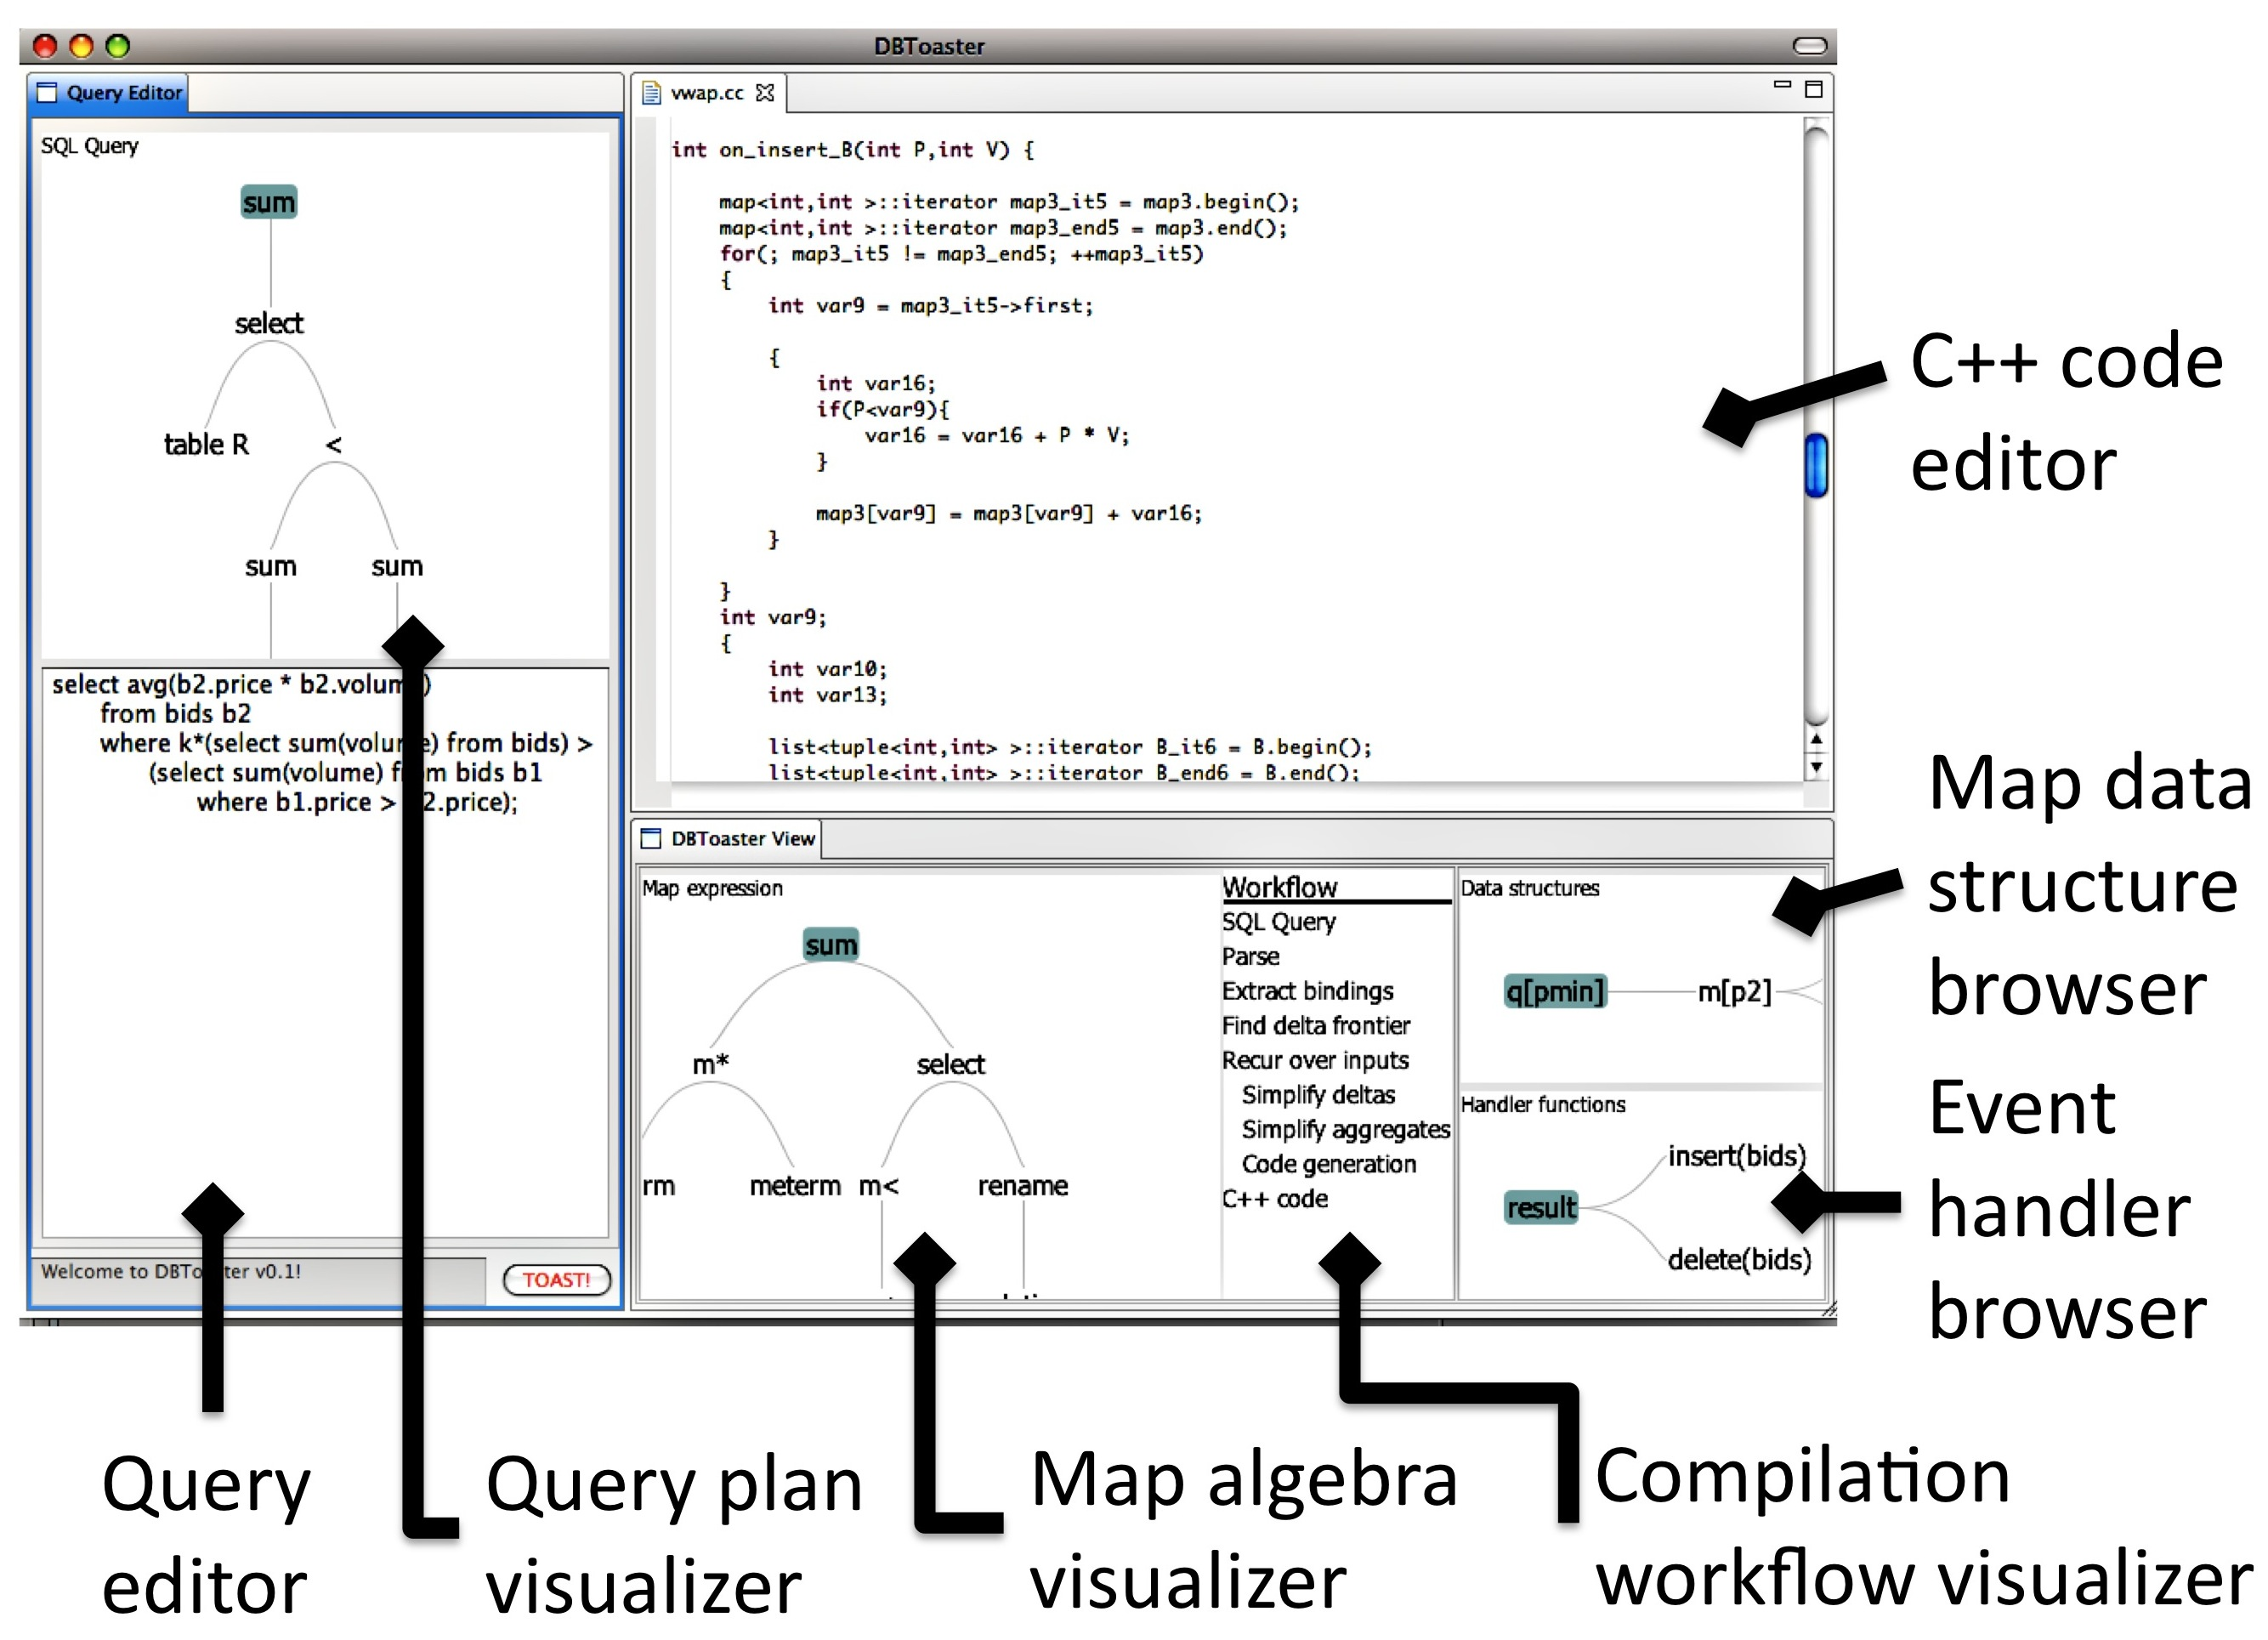
\includegraphics[scale=0.088]{figures/dbt-gui}
\end{center}

\vspace{-4mm}

\caption{\compiler\ compilation process visualization, displaying map algebra
transformations, generated code, and internal views that must be maintained.}
\label{fig:compilegui}
\end{figure}

The first of our two visualization tools (Figure~\ref{fig:compilegui} above)
conveys the compilation process to demo attendees. This tool first visually
displays a standard relational query plan, before illustrating the compiler
workflow in a step-by-step fashion, including map algebra simplifications and the
maps instantiated during compilation. We place particular emphasis on the
recursive nature of our compilation, demonstrating compilation of deltas on the
queries corresponding to our map data structures. At this point query compilation
is complete, and we utilize a pair of browser windows listing both the maps and
the event handling functions generated to allow access to arbitrary steps in the
compilation process, to aid in discussions with attendees. We also use a
debugging tool to provide step-by-step tracing of map maintenance when
processing a delta.
\comment{ Depending on the
demonstration progress, we may additionally include an example of a
JIT-compilation of the example query to demonstrate the potential for a limited
degree of adaptivity during query execution.
}

\begin{figure}[tb]
\begin{center}
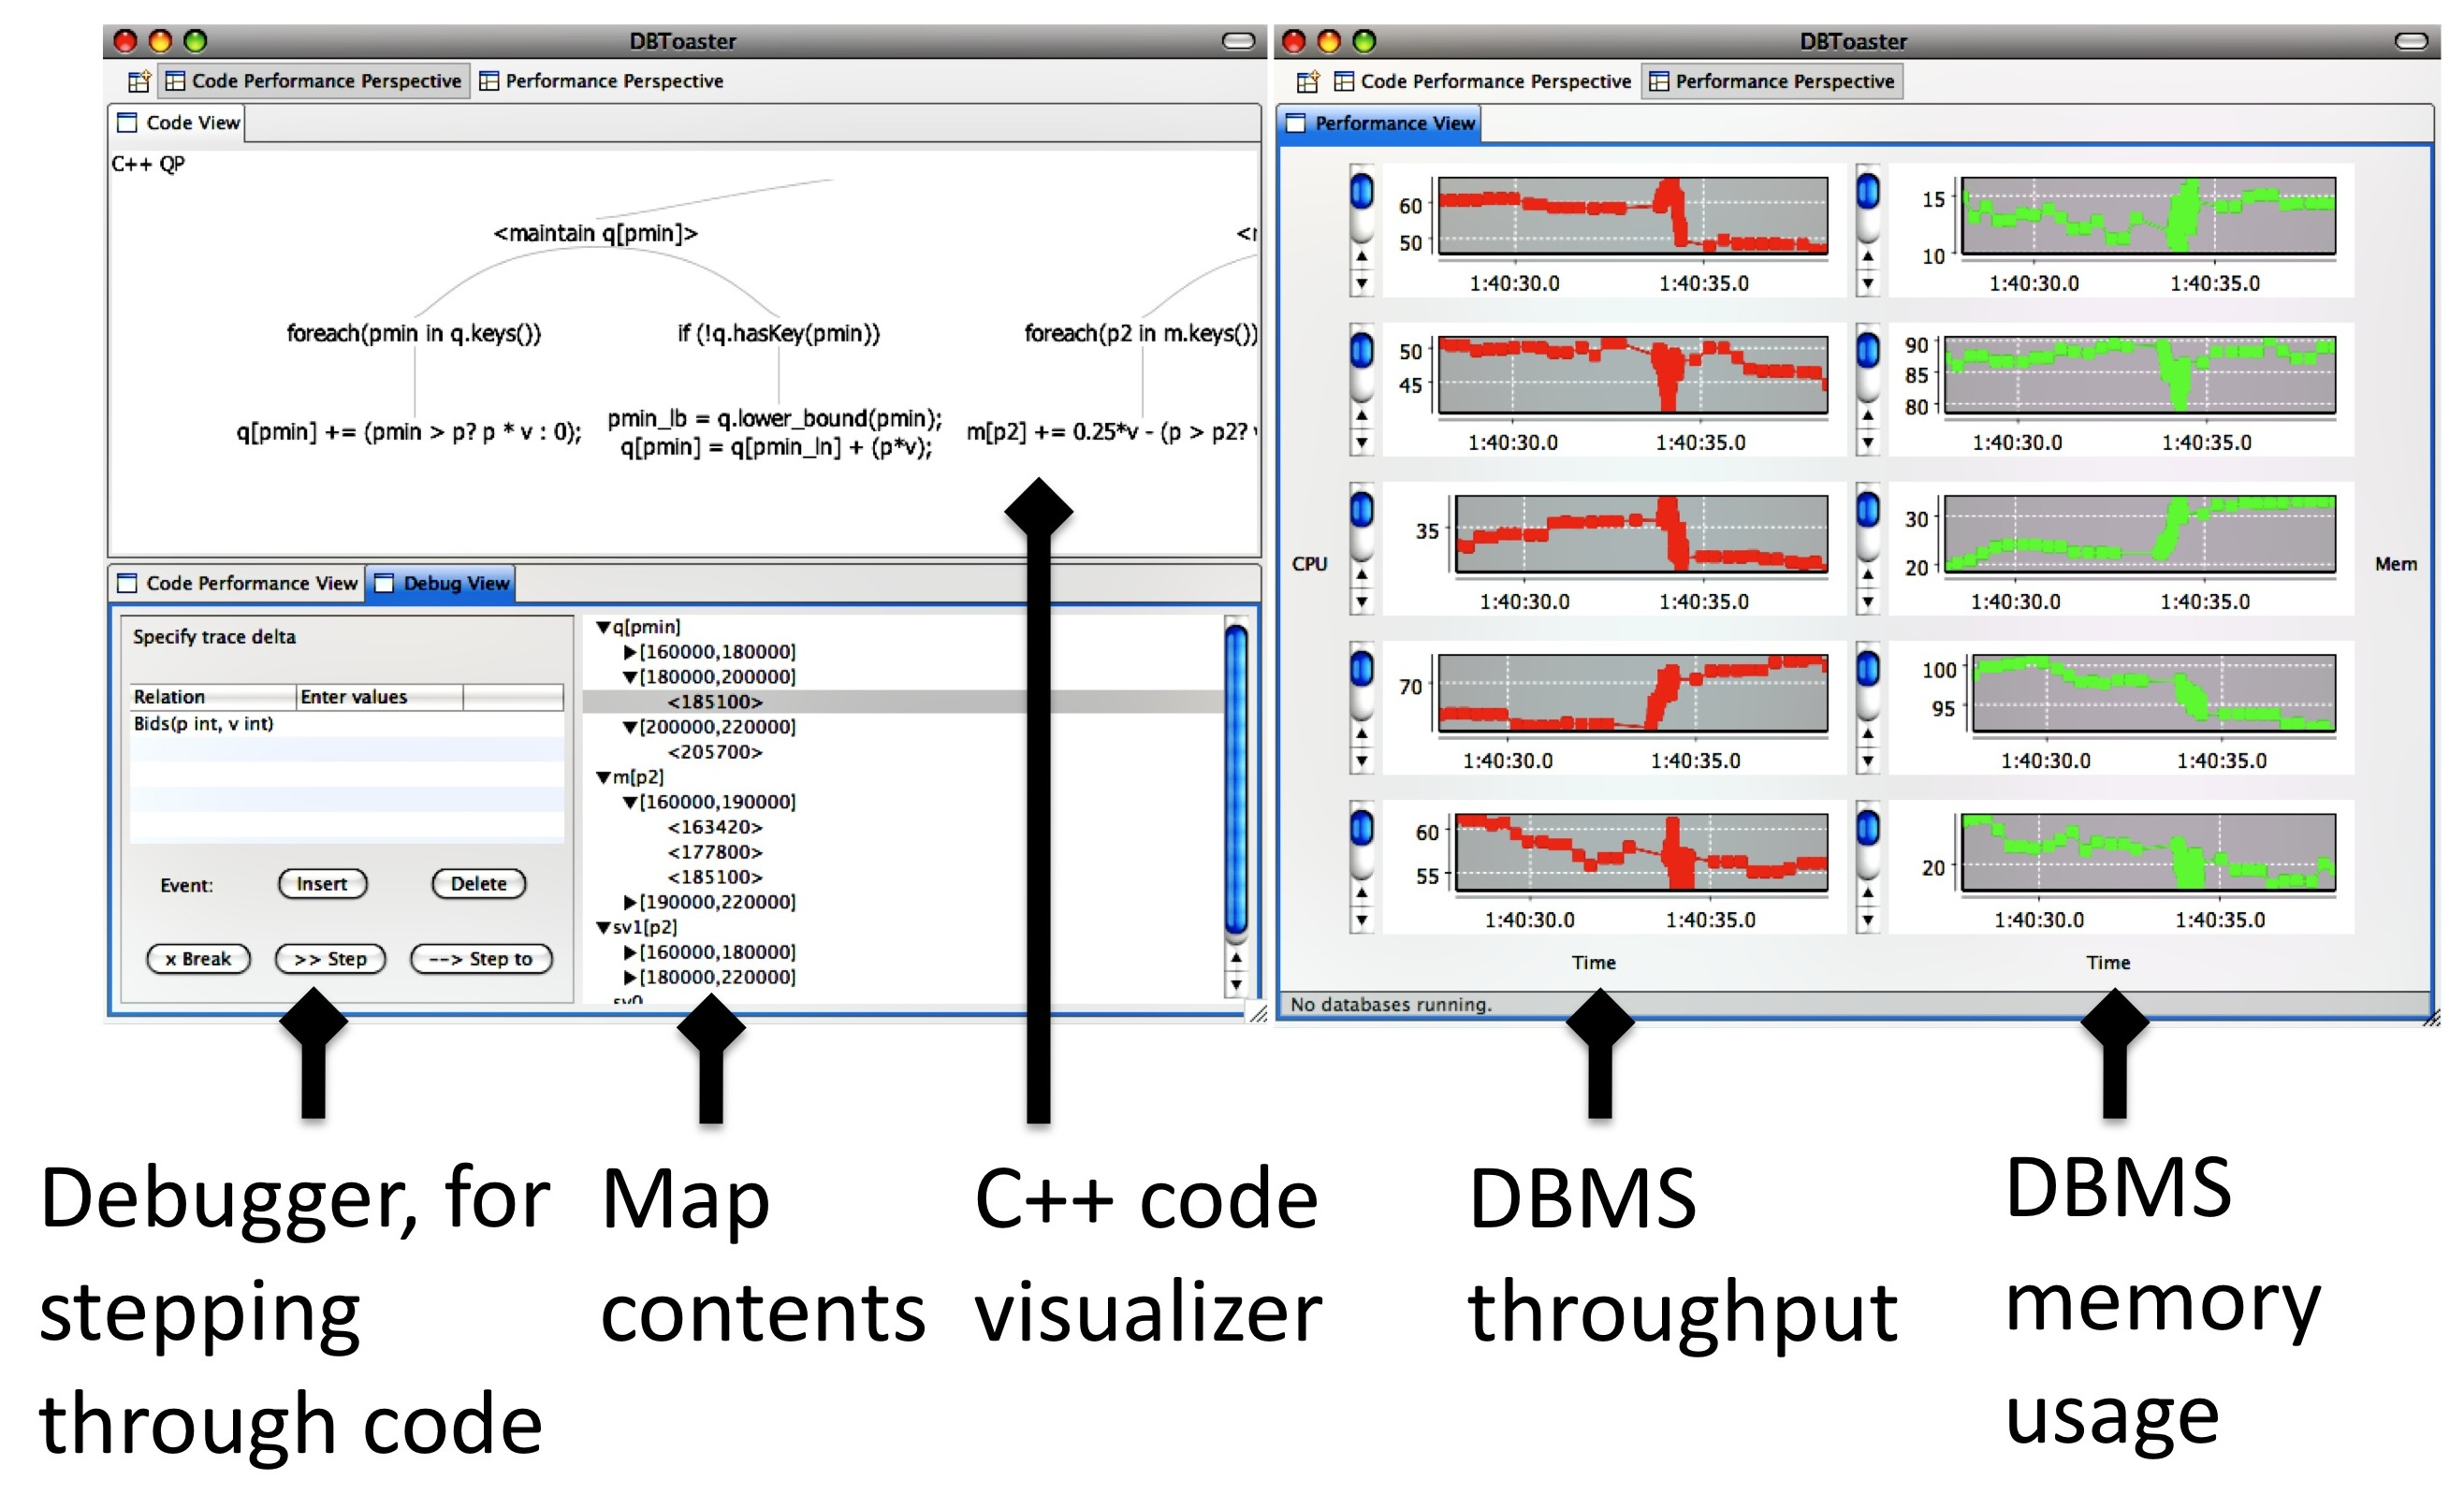
\includegraphics[scale=0.088]{figures/dbt-gui2}
\end{center}

\vspace{-4mm}

\caption{\compiler\ debugger supporting stepping and tracing query processing and
map maintenance, and performance visualizer for comparing against alternative
databases in the DBMS bakeoff.}
\label{fig:debugperfgui}
\end{figure}

\subsection{\compiler\ vs. DBMS* Bakeoff}
This demo also presents \compiler's competitiveness with a variety of database
tools, by performing a DBMS bakeoff. Our comparison points are PostgreSQL, a pure
Java main-memory DBMS (HSQLDB~\cite{hsqldb-url}), a commercial DBMS 'X', the
Stanford STREAM engine~\cite{motwani-cidr:03}, and a commerical stream processor
'Y'. We have a visualization tool to show the performance achieved by the each
database system including tuple throughput, memory usage and cache performance.
We also present detailed profiling of \compiler's compiled code breaking down its
overheads for each map, the binary size, and finally the compile time including
both the C++ generation and the subsequent compilation to a native binary. To
provide an entertaining audience experience, we run an audience challenge to find
queries both yielding the greatest performance over the other database engines in
the bakeoff, as well as queries that illustrate the poorest performance.
Attendees will be provided with two laptops at the demonstration booth to
experiment with queries, and encourage participation by displaying a leaderboard
of the running results.



%\footnotesize{
\bibliographystyle{abbrv}
\bibliography{ref}
%}

\end{document}
